\documentclass{article}

% Language setting
% Replace `english' with e.g. `spanish' to change the document language
\usepackage[english]{babel}

% Set page size and margins
% Replace `letterpaper' with`a4paper' for UK/EU standard size
\usepackage[letterpaper,top=2cm,bottom=2cm,left=3cm,right=3cm,marginparwidth=1.75cm]{geometry}

% Useful packages
\usepackage{amsmath}
\usepackage{graphicx}
\usepackage[colorlinks=true, allcolors=blue]{hyperref}

\title{Assignment 4. Bayesian Classifiers}
\author{Your name}

\begin{document}
\maketitle


Solve the following problems -- each problem on a separate page -- and submit to Gradescope for grading. 

\newpage
\section{Naive Bayes}
Given the following tiny dataset:

\begin{center}
\begin{tabular}{ |c|c|c|c| } 
 \hline
 A1 & A2 & A3 & Class \\
 \hline
1 & 0 & 1 & Yes \\ 
1 & 0 & 1 & Yes \\ 
0 & 1 & 1 & Yes \\ 
0 & 0 & 1 & Yes \\ 
1 & 0 & 0 & Yes \\ 
 \hline
\end{tabular}
\end{center}
\subsection {All probabilities [4 points]}
Compute all probabilities needed for a Naive Bayes classifier. Apply Laplace correction.
\subsection {Classify [2 points]}
Classify the following record $E=\left\{A1=0, A2=1, A3=0\right\}$ using Naïve Bayes classifier by comparing $P(yes|E)$ and $P(no|E)$.
\subsection {Probability of Yes/No [1 points]}
Give the actual values of both probabilities:

$P(yes|E) = ?$ 

$P(no| E) = ?$


Show your steps.

\newpage
\section{Bayesian Networks}
You are given the following topology of the Bayesian Belief Network:

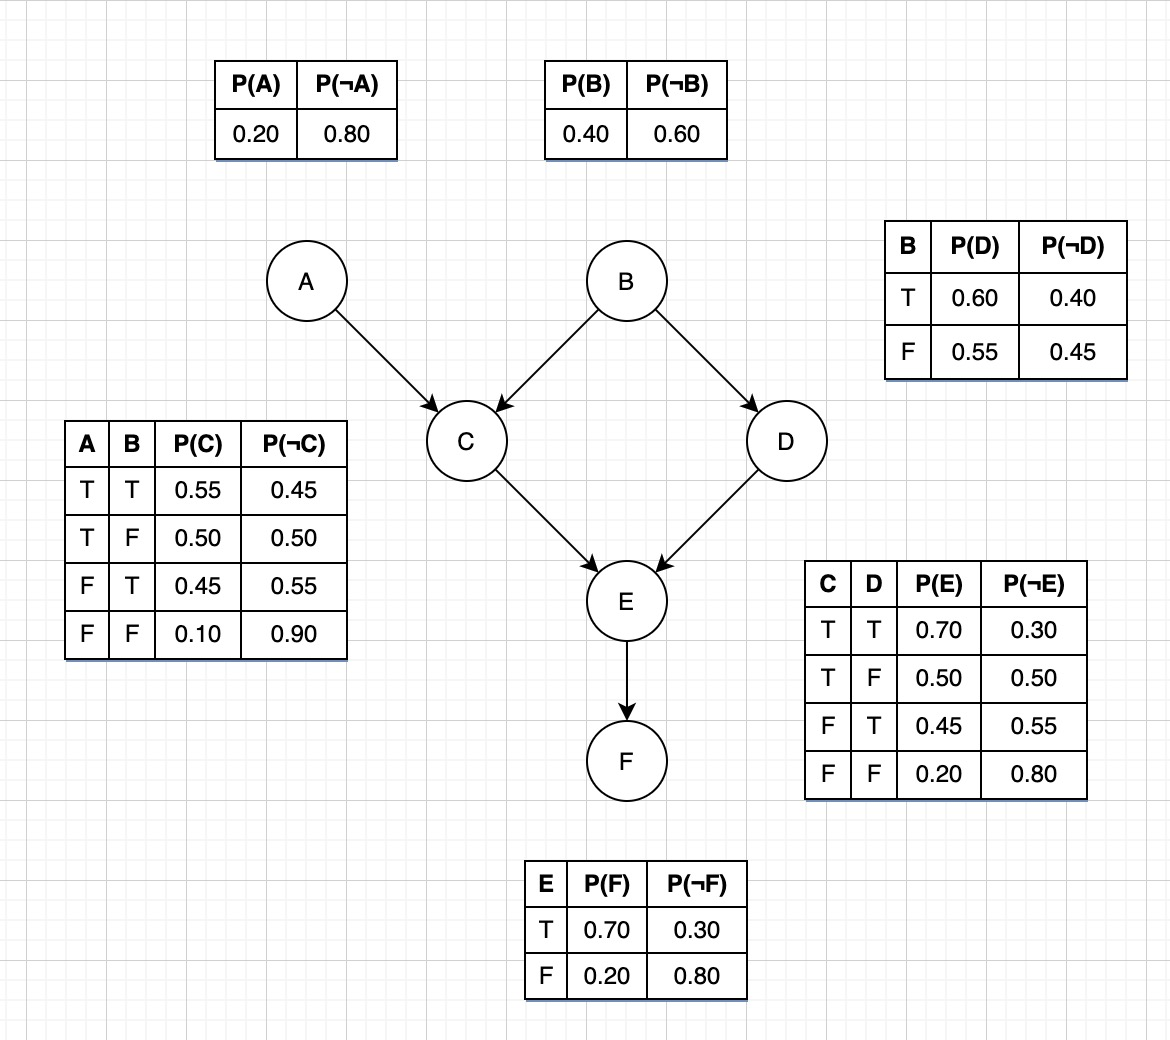
\includegraphics[width=\textwidth]{bayesian_network_full.jpg}


\subsection {Query 1 [3 points]}
Compute $P(c|a)$.

Nodes that we need to take into consideration (Markov blanket):

Computation of $P(c|a)$: 

$P(c|a) = ?$

\subsection {Query 2 [4 points]}
Compute $P(e|\neg c,b)$.

Nodes that we need to take into consideration (Markov blanket):

Computation of $P(e|\neg c,b)$: 

$P(e|\neg c,b) = ?$


\newpage
\section{My Own BBN [extra-credit]}
Get some fun for extra-credit! Design your own Bayesian Belief Network which will help you to answer some questions critically important in your life. Based on common sense and your life experience, define network topology, and fill in CPTs at each node. Finally come up with at least two queries that you would answer using your BBN.

You can insert an image of your network here (see the syntax for image in the previous section), and write as you normally do inside this document.

Optionally, because it is a for-fun and not-for-profit activity, you can work in any editor you like. If you selected this option, then at the end upload a final file (doc or pdf?) to canvas.

\end{document}



